\chapter{Introduction}\label{chapter:introduction}
Over the last two decades, the landscape of Computer Architecture has changed radically from sequential to parallel . Due to the limiting factors of technology we have moved from single core processors to multi core processors having a network interconnecting them. Traditionally, the approach of designing algorithms has been sequential, but designing algorithms in parallel is gaining more importance now to better utilize the computing power available at our disposal. Another important trend that has changed the face of computing is an enormous increase in the capabilities of the networks that connect computers with regards to speed, reliability etc. These trends make it feasible to develop applications that use physically distributed resources as if they were part of the same computer. A typical application of this sort may utilize processors on multiple remote computers, access a selection of remote databases, perform rendering on one or more graphics computers, and provide real-time output and control on a workstation. Computing on networked computers ("Distributed Computing") is not just a subfield of parallel computing as the basic task of developing programs that can run on many computers at once is a parallel computing problem. In this respect, the previously distinct worlds of parallel and distributed computing are converging.\\ \par
\noindent
As technology advances, we have newer problems or applications that demand larger computing capabilities which push the limits of technology giving rise to newer advancements. The performance of a computer depends directly on the time required to perform a basic operation and the number of these basic operations that can be performed concurrently. A metric used to quantify the performance of a computer is FLOPS (floating point operations per second). The time to perform a basic operation is ultimately limited by the "clock cycle" of the processor, that is, the time required to perform the most primitive operation. The term \textbf{\textit{High Performance Computing (HPC)}} refers to the practice of aggregating computing power (multiple nodes with processing units interconnected by a network in a certain toplogy) or the use of parallel processing for running advanced application programs efficiently, reliably and quickly. The term applies especially to systems that function above a \textbf{\textit{teraflop}} or \textbf{\textit{$10^{12}$}} floating-point operations per second. The term HPC is occasionally used as a synonym for Supercomputer that works at more than a \textbf{\textit{petaflop}} or \textbf{\textit{$10^{15}$}} floating-point operations per second. Future systems will reach \textbf{\textit{exaflop}} or \textbf{\textit{$10^{18}$}} floating-point operations per second. The most common users of HPC systems are scientific researchers, engineers, government agencies including the military, and academic institutions. In general, HPC systems can refer to Clusters, Supercomputers, Grid Computing etc. and they are usually used for running complex applications.\\ \par
\noindent
A \textbf{\textit{Batch System}} is used to manage the resources in a HPC System. It is a middleware that comprises of two major components namely the \textbf{\textit{Resource Manager}} and \textbf{\textit{Scheduler}}. The role of a Resource Manager is to act like a glue for a parallel computer to execute parallel jobs. It should make a parallel computer as easy to use as a Personal Computer (PC). A programming model such as \textbf{\textit{Message Passing Interface (MPI)}} for programming on distributed memory systems would typically be used to manage communications within a parallel program by using the MPI library functions. A Resource Manager allocates resources within a HPC system, launches and otherwise manages Jobs. Some of the examples of widely used open source as well as commercial resource managers are \textbf{\textit{SLURM, TORQUE, OMEGA, IBM Platform LSF}} etc. Together with a scheduler it is termed as a Batch System. The role of a job scheduler is to manage queue(s) of work when there is more work than resources. It supports complex scheduling algorithms which are optimized for network topology, energy efficiency, fair share scheduling, advanced reservations, preemption, gang scheduling (time-slicing jobs) etc. It also supports resource limits (by queue, user, group, etc.). Many batch systems provide both resource management and job scheduling within a single product (e.g. LSF) while others use distinct products(e.g. Torque Resource Manager and Moab Job Scheduler). Some other examples of Job Scheduling Systems are \textbf{\textit{LoadLeveler, OAR, Maui, SLURM etc.}}\\ \par
\noindent
Existing Batch Systems usually support only static allocation of resources to an application before they start which means the resources once allocated are fixed for the lifetime of the application. The complexity of applications have been growing, However, especially when we consider advanced techniques in Scientific Computing like \textbf{\textit{Adaptive Mesh Refinement (AMR)}} where applications exhibit complex behavior by changing their resource requirements during execution. The Batch Systems of today are not equipped to deal with such kind of complex applications in an intelligent manner apart from giving them the maximum number of resources before it starts that will result in a sheer wastage of resources leading to a poor resource utilization. In order to support such adaptive  applications at HPC centers there is an urgent need to investigate and implement extensions to existing resource management systems or develop an entirely new system. These supporting infrastructures must be able to handle the new kind of applications and the legacy ones intelligently keeping in mind that they should now be able to achieve much higher system utilization, throughput, energy efficiency etc. compared to their predecessors due to the elasticity of the applications.

\section{Invasive Computing}
Invasive Computing is a novel paradigm for the design and resource-aware programming of future parallel computing systems. It enables the programmer to write efficient resource aware programs. This approach can be used to allocate, execute on and free resources during execution of the program. The result is an adaptive application which can expand and shrink in the number of its resources at runtime. HPC infrastructures like clusters, supercomputers execute a vast variety of jobs, majority of which are parallel applications. These centers use intelligent resource management systems that should not only perform tasks of job management, resource management and scheduling but also satisfy important metrics like higher system utilization, job throughput and responsiveness. Traditionally, MPI applications are executed with a fixed number of MPI processes but with Invasive MPI applications they can evolve dynamically at runtime in the number of their MPI processes. This in turn supports advanced techniques like AMR where the working set size of applications change at runtime. Such kind of adaptive programming paradigms need to be complemented with intelligent resource management systems that can  achieve much higher system utilization, energy efficiency, throughput etc. compared to their predecessors due to elasticity of the applications.\par
\noindent
\\Under the collaborative research project funded by the \textbf{German Research Foundation (DFG)} in the \textbf{Transregional Collaborative Research Centre 89 (TRR89)}, research efforts are being made to investigate this Invasive Computing approach at different levels of abstraction right from the hardware up to the programming model and its applications. \textbf{Invasive MPI} is an effort towards invasive programming with MPI where the application programmer has MPI extensions available for specifying at certain safe points in the program, the possibility of changing the resource set of the application during runtime or adapt to the available resources during execution.
%%%%%%%
\section{Dynamic Resource Management}
Two of the most widely used resource managers on HPC systems are \textbf{SLURM} and \textbf{TORQUE}. The two major components in general of any sophisticated resource manager are the batch scheduler and the process manager. The Process Manager is responsible for launching the jobs on the allocated resources and managing them throughout their lifetime. Examples of process manager are \textbf{\textit{Hydra, SLURM Daemon (slurmd)}} etc. The process managers interact with the processes of a parallel application via the \textbf{Process Management Interface (PMI)}. In order to support Invasive Resource Management, The following components will be implemented: \textbf{\textit{iBSched}} (Batch Scheduler for Invasic Jobs) built as an extension into an existing batch system and \textbf{\textit{iRTSched}} (Invasive Distributed Run TIme Scheduler) similar to a controller daemon which will sit between the batch scheduler and the process manager. \textbf{SLURM} is the choice of an existing batch system on which this prototype will be implemented for demonstrating Invasive Computing and \ref{fig:1} shows a high level illustration of the architecture for such an Invasive Resource Management.\\ \\
\begin{figure}[!htbp]
\centering
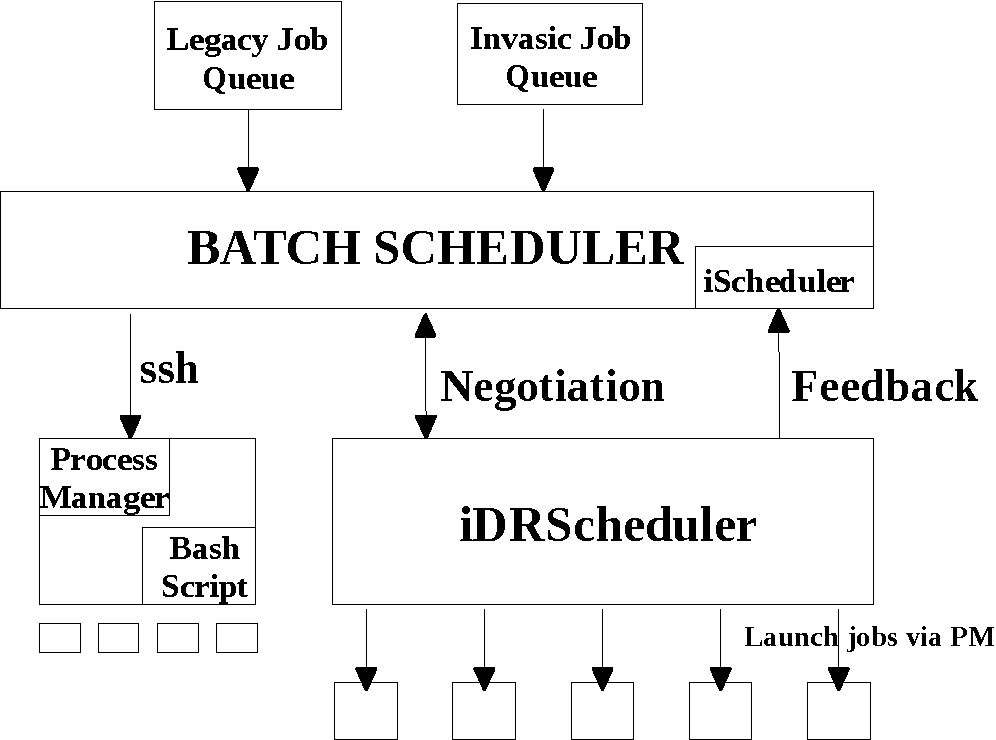
\includegraphics[width=1.0\textwidth, height=80mm]{./figures/architecture.pdf}
\caption{Invasive Resource Management Architecture}
\label{fig:1}
\end{figure}
\noindent
In addition to a job queue for legacy static jobs, we now have an additional job queue for invasic jobs. The objective of such a multi-level approach is to avoid modifying the existing system which will be a substantially large effort and rather have an independent component that caters specifically to Invasic Jobs. iRTSched is responsible for managing the resources present in the paritition used specifically for running Invasic Jobs. With this approach, the existing Legacy Jobs can be served via the existing batch scheduler and the new Invasic Jobs can be served by via iBSched and iRTSched. iRTSched talks to the iBSched via a protocol called the Negotiation protocol to receive Invasic Jobs dispatched from iBSched which it then launches for execution by performing some run time scheduling like pinning of jobs, expand/shrink etc.\\ \par
\noindent
The new components proposed in the architecture help achieve the objective of supporting dynamic resource management for invasic applications. iBSched is responsible for scheduling Invasic Jobs. The scheduling decisions are communicated via negotiation protocol to iRTSched and these decisions are basically job(s) selected via a scheduling algorithm to be submitted for execution. The decisions will be made on the basis of Resource Offers sent by iRTSched which creates these resource offers based on the state of the partition. Upon receiving a resource offer, iBSched will either accept it by selecting jobs from the queue that can be mapped to this offer or reject it. A Resource Offer can represent real or virtual resources because the iRTSched can also present a virtual view of resources in the hope of getting a mapping of jobs to offer that is more suitable to satisfy its local metrics such as resource utilization, power stability, energy efficiency etc. It can either accept or reject the mapping received from iBSched. Similar to iRTSched, the iBSched makes its decisions to optimize for certain local metrics such as high job throughput, reduced job waiting times, deadlines, priorities etc. This highlights the mismatching policies/metrics for which both the iRTSched and iBSched make their decisions on and hence both will be involved in some kind of a negotiation via the protocol to reach a common agreement. iRTSched is an independent entity introduced with the purpose of inter-operating with existing batch systems rather than replacing them with an entirely new one. It may be possible that in the future this component will not be a separate entitiy but will be built into the batch system itself.
%%%%%%%%%%%%%
\section{Document Structure}
This is end of the first section which gave an introduction to this Master Thesis and the kind of problem it deals with. The rest of this report is organized as follows:
\begin{itemize}
\item \textbf{\textit{Related Work:}} This section will briefly mention some of the earlier research efforts that have been made in the direction of batch job scheduling, runtime scheduling specifically to support adaptive applications and resource-aware programming paradigms to implement adaptive applications. 
\item \textbf{\textit{Invasive Computing:}} This section will first introduce the concept of invasive computing in brief and explain the motivation behind this concept. This is followed by an elaborate description of the traditional resource management approach in order to contrast it with the following section on invasive resource management that is necessary to support invasive computing. 
\item \textbf{\textit{Architecture:}} This section will present an abstraction of the complete system at a high level showing all the components and how they will interact with each other like a skeleton. It deals with what is being done and where is it being done but not how. This "how" is tackled in the following section of design.
\item \textbf{\textit{Design:}} This section will present the details on how we are building the system whose architecture was illustrated in the previous section. It deals with the internal details of the individual modules / components, flow charts and illustrations. It describes what it can do and what it cannot.
\item \textbf{\textit{Evaluation:}} This section will cover the evaluation of the work presented in this thesis. It will describe the approach used for evaluating the system in order to test its functionality, correctness and performance.
\item \textbf{\textit{Conclusion and Future Work:}} This last section concludes the report on this thesis with a highlight of what was successfully achieved along with the possible scope of what can be done as a part of future research work. This is followed by a list of some useful references that played an important role in the understanding of many of the concepts towards the realization of this project.
\end{itemize}
